\section{Un protocole d'échantillonnage aléatoire adaptatif}

\begin{frame}{Communication}{Propagation des modifications}

  Préserver la \textbf{cohérence à terme} des documents requière que tous les
  identifiants générés par la structure de séquences soient intégrés par tous
  les éditeurs.
  
  \vspace{0.5cm}
  
  Les éditeurs collaboratifs nécessitent un moyen de \textbf{communiquer} les
  changements effectués sur le document à tous les éditeurs impliqués dans
  l'édition.
  
  \vspace{0.5cm}

  \large
  \begin{itemize}
  \item [$\rightarrow$] \textbf{Dissémination d'information}
  \end{itemize}
  \vspace{0.5cm}
\end{frame}


\begin{frame}{Communication}{Diffusion épidémique}
  En \textbf{décentralisé}, la diffusion épidémique de messages constitue une
  manière efficace de disséminer l'information. Les messages parviennent à tous
  les pairs sans que ceux-ci ne connaissent tous les membres du réseau.

  \vspace{0.5cm}

  Fonctionnement : chaque pair possède une vue partielle du réseau.
  \begin{enumerate}
  \uncover<2->{\item un pair souhaitant diffuser un message l'envoie à sa vue partielle;}
  \uncover<3->{\item chaque pair recevant un tel message le diffuse à sa vue partielle;}
  \uncover<4->{\item condition d'arrêt : le message a déjà été reçu auparavant.}
  \end{enumerate}

  \begin{minipage}{0.45\textwidth}
    \begin{center}
      \begin{tikzpicture}[scale=1]

\newcommand\X{40pt}
\newcommand\Y{-15pt}

\draw[->] (0*\X, 0*\Y) -- (-5+1*\X,-3*\Y);
\draw[->](0*\X, 0*\Y) -- (-5+1*\X,-0*\Y);
\draw[->] (0*\X, 0*\Y) -- (-5+1*\X, 3*\Y);

% \only<2>\draw[->, very thick] (0*\X, 0*\Y) -- (-5+1*\X,-3*\Y);
% \only<2>\draw[->, very thick](0*\X, 0*\Y) -- (-5+1*\X,-0*\Y);
% \only<2>\draw[->, very thick] (0*\X, 0*\Y) -- (-5+1*\X, 3*\Y);


\draw[->] (1*\X, 3*\Y) -- (-5+2*\X, 4*\Y);
\draw[->] (1*\X, 3*\Y) -- (-5+2*\X, 3*\Y);
\draw[->] (1*\X, 3*\Y) -- (-5+2*\X, 2*\Y);

\draw[->] (1*\X, 0*\Y) -- (-5+2*\X, 1*\Y);
\draw[->] (1*\X, 0*\Y) -- (-5+2*\X, 0*\Y);
\draw[->] (1*\X, 0*\Y) -- (-5+2*\X,-1*\Y);

\draw[->] (1*\X,-3*\Y) -- (-5+2*\X,-2*\Y);
\draw[->] (1*\X,-3*\Y) -- (-5+2*\X,-3*\Y);
\draw[->] (1*\X,-3*\Y) -- (-5+2*\X,-4*\Y);

% \only<3>\draw[->, very thick] (1*\X, 3*\Y) -- (-5+2*\X, 4*\Y);
% \only<3>\draw[->, very thick] (1*\X, 3*\Y) -- (-5+2*\X, 3*\Y);
% \only<3>\draw[->, very thick] (1*\X, 3*\Y) -- (-5+2*\X, 2*\Y);

% \only<3>\draw[->, very thick] (1*\X, 0*\Y) -- (-5+2*\X, 1*\Y);
% \only<3>\draw[->, very thick] (1*\X, 0*\Y) -- (-5+2*\X, 0*\Y);
% \only<3>\draw[->, very thick] (1*\X, 0*\Y) -- (-5+2*\X,-1*\Y);

% \only<3>\draw[->, very thick] (1*\X,-3*\Y) -- (-5+2*\X,-2*\Y);
% \only<3>\draw[->, very thick] (1*\X,-3*\Y) -- (-5+2*\X,-3*\Y);
% \only<3>\draw[->, very thick] (1*\X,-3*\Y) -- (-5+2*\X,-4*\Y);


%\draw[<-, very thick, color=white] (5+1*\X, 5-3*\Y)to[out=90,in=140](-5+2*\X, 5-4*\Y);
%\draw[<-] (5+1*\X, 5-3*\Y)to[out=90,in=140](-5+2*\X, 5-4*\Y);
% \only<4>\draw[<-, very thick] (5+1*\X, 5-3*\Y)to[out=90,in=140](-5+2*\X, 5-4*\Y);
% \only<4>{\draw[fill=white, very thick] ( 2*\X, -4*\Y) node{$e_a$} +(-5pt,-5pt) rectangle +(5pt,5pt);}

%% ea --- ec
\draw[->](2*\X, -4*\Y) -- (3*\X, 5-4*\Y);
\draw[->](2*\X, -4*\Y) -- (3*\X, -5-4*\Y);
\draw[->](2*\X, -4*\Y) -- (3*\X, -0-4*\Y);
%\draw[->](2*\X, -4*\Y) -- (3*\X,  5-4*\Y);

\draw[->](2*\X, -3*\Y) -- (3*\X, -5-3*\Y);
\draw[->](2*\X, -3*\Y) -- (3*\X, -0-3*\Y);
\draw[->](2*\X, -3*\Y) -- (3*\X,  5-3*\Y);

\draw[->](2*\X, -2*\Y) -- (3*\X, -5-2*\Y);
\draw[->](2*\X, -2*\Y) -- (3*\X, -0-2*\Y);
\draw[->](2*\X, -2*\Y) -- (3*\X,  5-2*\Y);

%% ed --- ef
\draw[->](2*\X, -1*\Y) -- (3*\X, -5-1*\Y);
\draw[->](2*\X, -1*\Y) -- (3*\X, -0-1*\Y);
\draw[->](2*\X, -1*\Y) -- (3*\X,  5-1*\Y);

\draw[->](2*\X, -0*\Y) -- (3*\X, -5-0*\Y);
\draw[->](2*\X, -0*\Y) -- (3*\X, -0-0*\Y);
\draw[->](2*\X, -0*\Y) -- (3*\X,  5-0*\Y);

\draw[->](2*\X, 1*\Y) -- (3*\X, -5+1*\Y);
\draw[->](2*\X, 1*\Y) -- (3*\X, -0+1*\Y);
\draw[->](2*\X, 1*\Y) -- (3*\X,  5+1*\Y);

%% eg --- ei
\draw[->](2*\X, 2*\Y) -- (3*\X, -5+2*\Y);
\draw[->](2*\X, 2*\Y) -- (3*\X, -0+2*\Y);
\draw[->](2*\X, 2*\Y) -- (3*\X,  5+2*\Y);

\draw[->](2*\X, 3*\Y) -- (3*\X, -5+3*\Y);
\draw[->](2*\X, 3*\Y) -- (3*\X, -0+3*\Y);
\draw[->](2*\X, 3*\Y) -- (3*\X,  5+3*\Y);

\draw[->](2*\X, 4*\Y) -- (3*\X, -5+4*\Y);
\draw[->](2*\X, 4*\Y) -- (3*\X, -0+4*\Y);
\draw[->](2*\X, 4*\Y) -- (3*\X,  5+4*\Y);


%% ea --- ec
% \only<4>\draw[->, very thick](2*\X, -4*\Y) -- (3*\X, -5-4*\Y);
% \only<4>\draw[->, very thick](2*\X, -4*\Y) -- (3*\X, -0-4*\Y);
% %\only<4>\draw[->, very thick](2*\X, -4*\Y) -- (3*\X,  5-4*\Y);

% \only<4>\draw[->, very thick](2*\X, -3*\Y) -- (3*\X, -5-3*\Y);
% \only<4>\draw[->, very thick](2*\X, -3*\Y) -- (3*\X, -0-3*\Y);
% \only<4>\draw[->, very thick](2*\X, -3*\Y) -- (3*\X,  5-3*\Y);

% \only<4>\draw[->, very thick](2*\X, -2*\Y) -- (3*\X, -5-2*\Y);
% \only<4>\draw[->, very thick](2*\X, -2*\Y) -- (3*\X, -0-2*\Y);
% \only<4>\draw[->, very thick](2*\X, -2*\Y) -- (3*\X,  5-2*\Y);

% %% ed --- ef
% \only<4>\draw[->, very thick](2*\X, -1*\Y) -- (3*\X, -5-1*\Y);
% \only<4>\draw[->, very thick](2*\X, -1*\Y) -- (3*\X, -0-1*\Y);
% \only<4>\draw[->, very thick](2*\X, -1*\Y) -- (3*\X,  5-1*\Y);

% \only<4>\draw[->, very thick](2*\X, -0*\Y) -- (3*\X, -5-0*\Y);
% \only<4>\draw[->, very thick](2*\X, -0*\Y) -- (3*\X, -0-0*\Y);
% \only<4>\draw[->, very thick](2*\X, -0*\Y) -- (3*\X,  5-0*\Y);

% \only<4>\draw[->, very thick](2*\X, 1*\Y) -- (3*\X, -5+1*\Y);
% \only<4>\draw[->, very thick](2*\X, 1*\Y) -- (3*\X, -0+1*\Y);
% \only<4>\draw[->, very thick](2*\X, 1*\Y) -- (3*\X,  5+1*\Y);

% %% eg --- ei
% \only<4>\draw[->, very thick](2*\X, 2*\Y) -- (3*\X, -5+2*\Y);
% \only<4>\draw[->, very thick](2*\X, 2*\Y) -- (3*\X, -0+2*\Y);
% \only<4>\draw[->, very thick](2*\X, 2*\Y) -- (3*\X,  5+2*\Y);

% \only<4>\draw[->, very thick](2*\X, 3*\Y) -- (3*\X, -5+3*\Y);
% \only<4>\draw[->, very thick](2*\X, 3*\Y) -- (3*\X, -0+3*\Y);
% \only<4>\draw[->, very thick](2*\X, 3*\Y) -- (3*\X,  5+3*\Y);

% \only<4>\draw[->, very thick](2*\X, 4*\Y) -- (3*\X, -5+4*\Y);
% \only<4>\draw[->, very thick](2*\X, 4*\Y) -- (3*\X, -0+4*\Y);
% \only<4>\draw[->, very thick](2*\X, 4*\Y) -- (3*\X,  5+4*\Y);



\draw[fill=white] ( 0*\X, 0*\Y) node{$e$} +(-5pt,-5pt) rectangle +(5pt,5pt);
% \only<2>{\draw[fill=white, very thick] ( 0*\X, 0*\Y) node{$e$} +(-5pt,-5pt) rectangle +(5pt,5pt);}

\draw[fill=white] ( 1*\X,-3*\Y) node{$e_1$} +(-5pt,-5pt) rectangle +(5pt,5pt);
\draw[fill=white] ( 1*\X, 0*\Y) node{$e_2$} +(-5pt,-5pt) rectangle +(5pt,5pt);
\draw[fill=white] ( 1*\X, 3*\Y) node{$e_3$} +(-5pt,-5pt) rectangle +(5pt,5pt);

% \only<3>{\draw[fill=white, very thick] ( 1*\X,-3*\Y) node{$e_1$} +(-5pt,-5pt) rectangle +(5pt,5pt);}
% \only<3>{\draw[fill=white, very thick] ( 1*\X, 0*\Y) node{$e_2$} +(-5pt,-5pt) rectangle +(5pt,5pt);}
% \only<3>{\draw[fill=white, very thick] ( 1*\X, 3*\Y) node{$e_3$} +(-5pt,-5pt) rectangle +(5pt,5pt);}


\draw[fill=white] ( 2*\X, -4*\Y) node{$e_a$} +(-5pt,-5pt) rectangle +(5pt,5pt);
\draw[fill=white] ( 2*\X, -3*\Y) node{$e_b$} +(-5pt,-5pt) rectangle +(5pt,5pt);
\draw[fill=white] ( 2*\X, -2*\Y) node{$e_c$} +(-5pt,-5pt) rectangle +(5pt,5pt);

\draw[fill=white] ( 2*\X, -1*\Y) node{$e_d$} +(-5pt,-5pt) rectangle +(5pt,5pt);
\draw[fill=white] ( 2*\X,  0*\Y) node{$e_e$} +(-5pt,-5pt) rectangle +(5pt,5pt);
\draw[fill=white] ( 2*\X,  1*\Y) node{$e_f$} +(-5pt,-5pt) rectangle +(5pt,5pt);

\draw[fill=white] ( 2*\X,  2*\Y) node{$e_g$} +(-5pt,-5pt) rectangle +(5pt,5pt);
\draw[fill=white] ( 2*\X,  3*\Y) node{$e_h$} +(-5pt,-5pt) rectangle +(5pt,5pt);
\draw[fill=white] ( 2*\X,  4*\Y) node{$e_i$} +(-5pt,-5pt) rectangle +(5pt,5pt);

% \only<4>{\draw[fill=white, very thick] ( 2*\X, -4*\Y) node{$e_a$} +(-5pt,-5pt) rectangle +(5pt,5pt);}
% \only<4>{\draw[fill=white, very thick] ( 2*\X, -3*\Y) node{$e_b$} +(-5pt,-5pt) rectangle +(5pt,5pt);}
% \only<4>{\draw[fill=white, very thick] ( 2*\X, -2*\Y) node{$e_c$} +(-5pt,-5pt) rectangle +(5pt,5pt);}

% \only<4>{\draw[fill=white, very thick] ( 2*\X, -1*\Y) node{$e_d$} +(-5pt,-5pt) rectangle +(5pt,5pt);}
% \only<4>{\draw[fill=white, very thick] ( 2*\X,  0*\Y) node{$e_e$} +(-5pt,-5pt) rectangle +(5pt,5pt);}
% \only<4>{\draw[fill=white, very thick] ( 2*\X,  1*\Y) node{$e_f$} +(-5pt,-5pt) rectangle +(5pt,5pt);}

% \only<4>{\draw[fill=white, very thick] ( 2*\X,  2*\Y) node{$e_g$} +(-5pt,-5pt) rectangle +(5pt,5pt);}
% \only<4>{\draw[fill=white, very thick] ( 2*\X,  3*\Y) node{$e_h$} +(-5pt,-5pt) rectangle +(5pt,5pt);}
% \only<4>{\draw[fill=white, very thick] ( 2*\X,  4*\Y) node{$e_i$} +(-5pt,-5pt) rectangle +(5pt,5pt);}



\end{tikzpicture}
    \end{center}
  \end{minipage}
  \hfill
  \begin{minipage}{0.5\textwidth}
    \large
    \begin{itemize}
      \uncover<5->{\item [$\rightarrow$] \textbf{Comment configurer la taille
          des vues partielles et les peupler ?}}
    \end{itemize}
  \end{minipage}

\end{frame}


\begin{frame}{Communication}{Contexte Web}
  
  \begin{minipage}{0.69\textwidth}
    Le contexte \textbf{Web} pousse à la \textbf{centralisation :}
    \begin{itemize}
    \item problèmes de \textbf{confidentialité}, \textbf{censure}, etc.
    \uncover<2->{\item problèmes de passage à l'échelle, notamment en \textbf{nombre de
        collaborateurs};}
    \uncover<3->{\item problèmes de \textbf{résilience} aux pannes.}
    \end{itemize}
  \end{minipage}
  \hfill
  \begin{minipage}{0.3\textwidth}
    
\includegraphics[width=0.7\textwidth]{img/www.png}
  \end{minipage}

  \vspace{0.75cm}
  

  \begin{minipage}{0.32\textwidth}
    \begin{center}
      \begin{tikzpicture}
        \node[visible on=<1-3>]
        {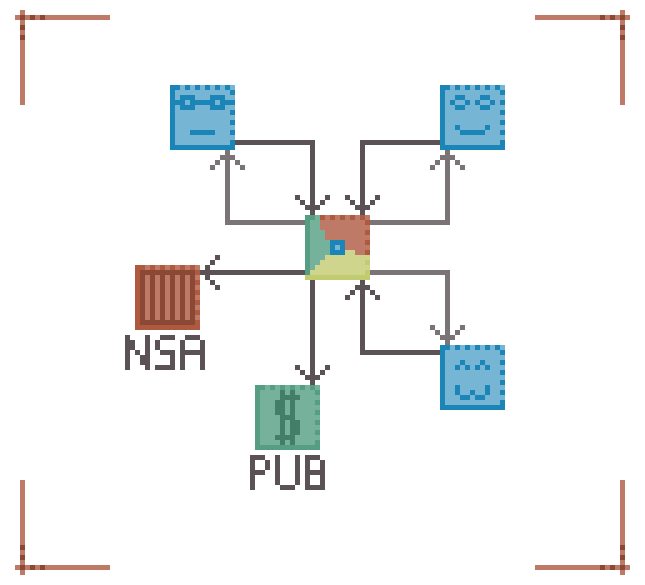
\includegraphics[width=0.95\textwidth]{img/centralizedethicproblems.png}};
      \end{tikzpicture}
    \end{center}
  \end{minipage}
  \begin{minipage}{0.32\textwidth}
    \begin{center}
      \begin{tikzpicture}
        \node[visible on=<2-3>]
        {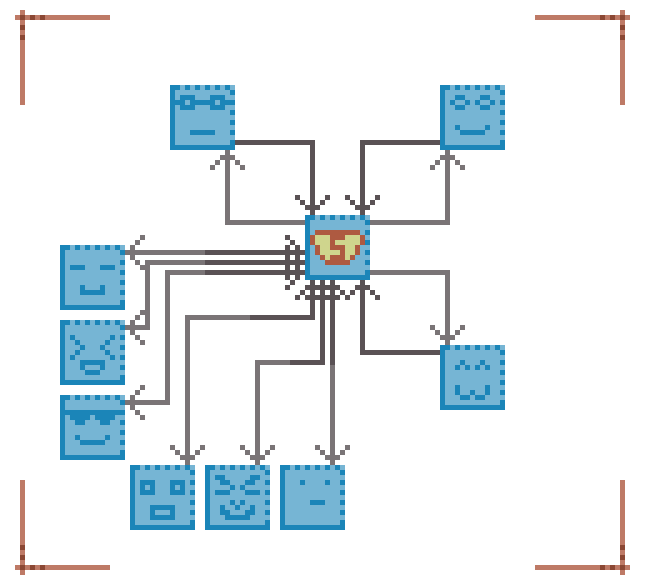
\includegraphics[width=0.95\textwidth]{img/centralizedcpuproblems.png}};
      \end{tikzpicture}
    \end{center}
  \end{minipage}
  \begin{minipage}{0.32\textwidth}
    \begin{center}
      \begin{tikzpicture}
        \node[visible on=<3-3>]
        {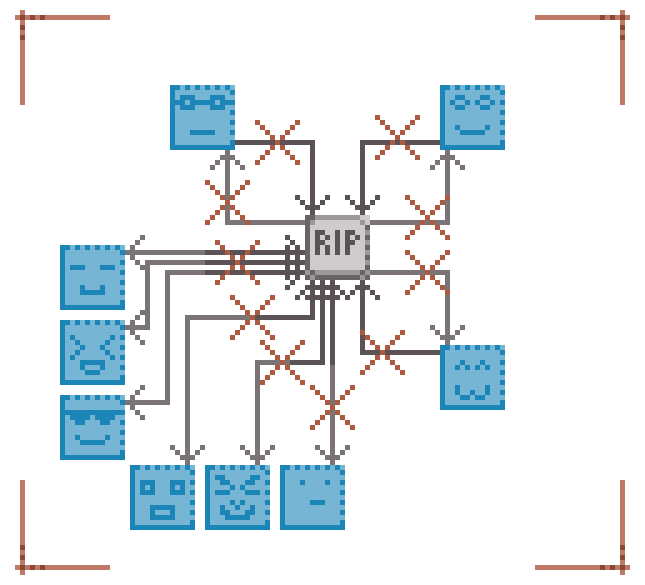
\includegraphics[width=0.95\textwidth]{img/centralizedscalabilityproblems.png}};
      \end{tikzpicture}        
    \end{center}
  \end{minipage}
\end{frame}


\begin{frame}{Communication}{Possible grâce à WebRTC}

  Les navigateur Web ne sont plus seulement des clients mais aussi des
  \textbf{serveurs}. En revanche, 
  
  \vspace{0.5cm}
  
  \begin{minipage}{0.6\textwidth}
    \begin{itemize}
    \item \textbf{ni adresses ni routes};
    \item les connexions sont \textbf{coûteuses} et sujettes aux
      \textbf{defaillances};
    \item \textbf{capacités hétérogènes et parfois limités} des outils de
      navigation;
    \item le contexte Web expose aux \textbf{pics soudains de popularité.}
    \end{itemize}
  \end{minipage}
  \hfill
  \begin{minipage}{0.3\textwidth}
    
\includegraphics[width=0.7\textwidth]{img/webrtc.png}
  \end{minipage}

  \vspace{0.5cm}


  \begin{minipage}{0.6\textwidth}
    Création d'un réseau :
    \begin{itemize}
    \uncover<2->{\item Un \textbf{serveur sert de médiateur} à la connexion initiale;}
    \uncover<3->{\item Les pairs \textbf{deviennent des médiateurs} du réseau;}
    \uncover<4>{\item Réseau de trois membres avec connexions directes.}
    \end{itemize}
  \end{minipage}
  \begin{minipage}{0.3\textwidth}
    \begin{center}
      
\begin{tikzpicture}[scale=1.1]

\newcommand\X{40pt};
\newcommand\Y{15pt};

\draw( 1.7*\X, 0); %% spacing
\draw(-1.7*\X, 0); %% spacing

\draw[fill=white,very thick](0*\X, 0*\Y) 
node{serveur de signalement} +(-45pt,-5pt) rectangle +(45pt,5pt);

\small
\only<2>{\draw[->,dashed, very thick](-5 -1*\X, 5-2*\Y) --
node[anchor=east]{1} (-20pt,-5pt);
\draw[<-,dashed, very thick]( 5 -1*\X, 5-2*\Y) --
node[anchor=west]{4} (-10pt,-5pt);

\draw[<-,dashed, very thick](-5pt,  5-3*\Y) --
node[anchor=east]{2}(-5pt,-5pt);
\draw[->,dashed, very thick](5pt , 5-3*\Y) --
node[anchor=west]{3} (5pt,-5pt);}


\draw[fill=white]
(-1*\X,-2*\Y) node{$n_1$} +(-5pt,-5pt) rectangle +(5pt,5pt);
\draw[fill=white]
(0*\X, -3*\Y) node{$n_2$} +(-5pt,-5pt) rectangle +(5pt,5pt);
\draw[fill=white] (1*\X, -2*\Y) node{$n_3$} +(-5pt,-5pt) rectangle +(5pt,5pt);


\small
\only<3>{
\draw[<->, very thick](5-1*\X,-2*\Y)--
node[anchor=south]{1$\rightarrow$}
node[anchor=north]{$\leftarrow$4}(-5pt,-3*\Y);
\draw[<->, very thick](5pt,-3*\Y)--
node[anchor=south]{2$\rightarrow$}
node[anchor=north]{$\leftarrow$3}(-5+1*\X,-2*\Y);
}


\only<4>{
\draw[<->](5-1*\X,-2*\Y)--(-5pt,-3*\Y);
\draw[<->](5pt,-3*\Y)--(-5+1*\X,-2*\Y);
\draw[<->, very thick](5 - 1*\X, 2.5 -2*\Y)--(-5+1*\X, 2.5 -2*\Y);
}


\end{tikzpicture}

    \end{center}
  \end{minipage}

\end{frame}


\begin{frame}{Communication}{Définition du problème}

\begin{problem}
  \label{net:problem:properties}
  Soit $t$ une unité de temps arbitraire, soit $\mathcal{N}^t$ l'ensemble des
  membres non-byzantins du réseau à un instant $t$ et soit $P_i^t$ la vue
  partielle du nœud $n_i \in \mathcal{N}^t$. Un protocole d'échantillonnage
  aléatoire de pairs efficace doit assurer les propriétés suivantes :
  \begin{enumerate}
  \item Taille des vues partielles : \hfill $\forall n_i \in \mathcal{N}^t$,
    $|P_i^t| \approx \mathcal{O}(\ln |\mathcal{N}^t|)$
  \item Établissement de connexion : \hfill $\mathcal{O}(1)$
%  \item \TODO{Convergence}
  \end{enumerate}
\end{problem}

\end{frame}
